\documentclass{standalone}
\usepackage{tikz}
\usetikzlibrary{patterns}
\usetikzlibrary{positioning}
\usetikzlibrary{patterns, positioning}
\usetikzlibrary{shapes.misc}
\usepackage[outline]{contour}
\contourlength{1.5pt} 


\begin{document}
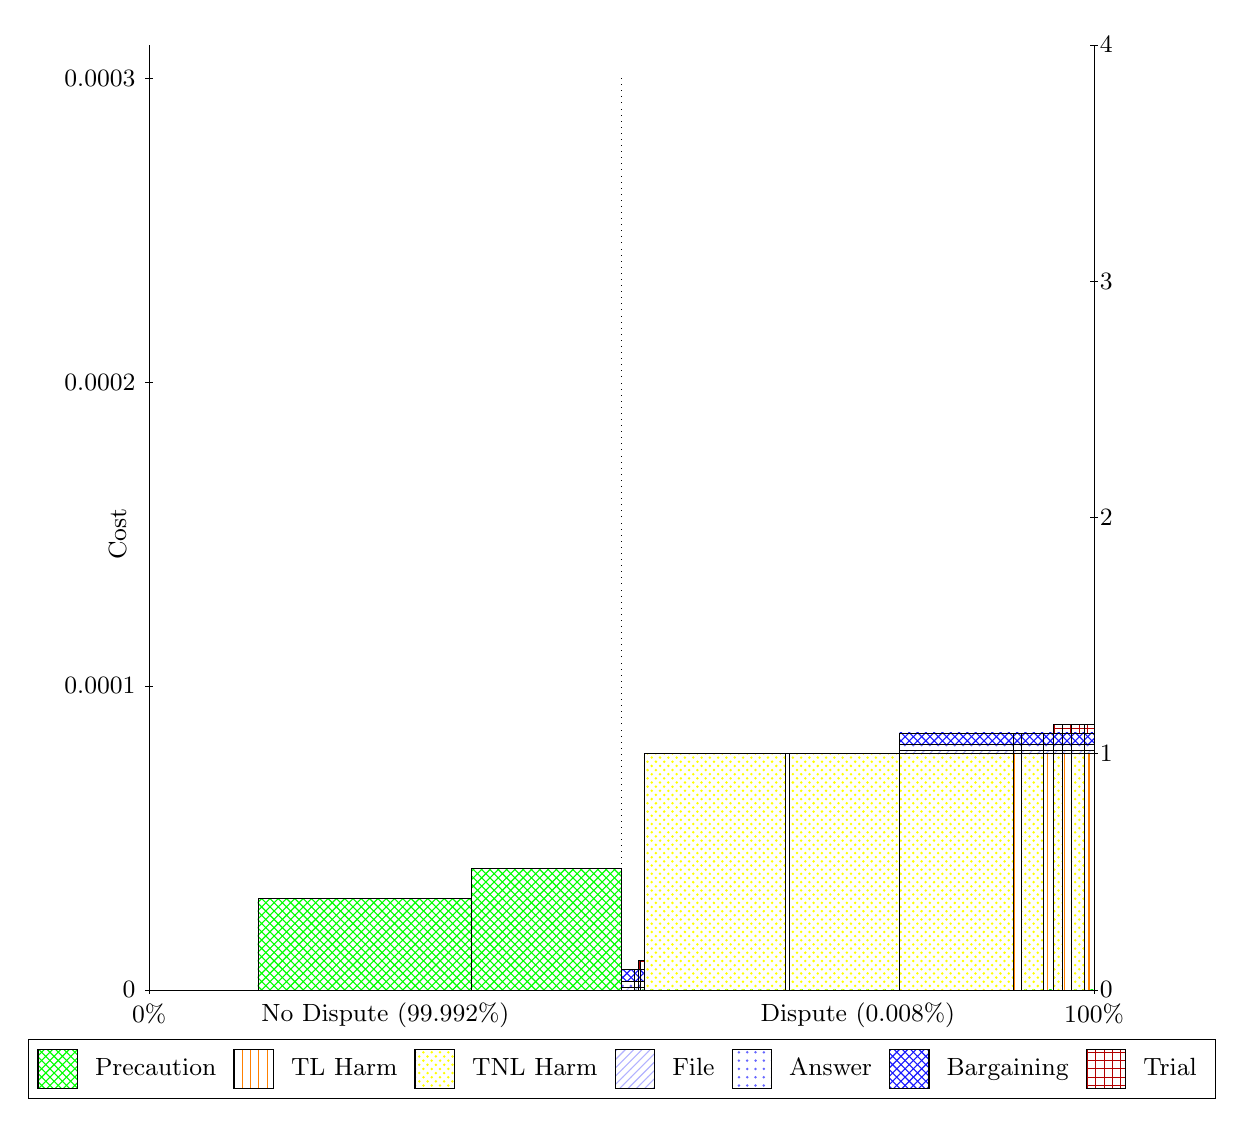
\begin{tikzpicture}
\draw[pattern=crosshatch, pattern color=green,draw=black,very thin] (2.8801,2.5) rectangle (5.5912,3.6579);
\draw[pattern=crosshatch, pattern color=green,draw=black,very thin] (5.5912,2.5) rectangle (7.5,4.0438);
\draw[pattern=north east lines, pattern color=blue!30,draw=black,very thin] (7.5,2.5) rectangle (7.6553,2.5375);
\draw[pattern=dots,  pattern color=blue!60,draw=black,very thin] (7.5,2.5375) rectangle (7.6553,2.6125);
\draw[pattern=crosshatch,      pattern color=blue!90,draw=black,very thin] (7.5,2.6125) rectangle (7.6553,2.7625);
\draw[pattern=crosshatch, pattern color=green,draw=black,very thin] (7.6553,2.5) rectangle (7.7147,2.5001);
\draw[pattern=north east lines, pattern color=blue!30,draw=black,very thin] (7.6553,2.5001) rectangle (7.7147,2.5376);
\draw[pattern=dots,  pattern color=blue!60,draw=black,very thin] (7.6553,2.5376) rectangle (7.7147,2.6126);
\draw[pattern=crosshatch,      pattern color=blue!90,draw=black,very thin] (7.6553,2.6126) rectangle (7.7147,2.7626);
\draw[pattern=north east lines, pattern color=blue!30,draw=black,very thin] (7.7147,2.5) rectangle (7.737,2.5375);
\draw[pattern=dots,  pattern color=blue!60,draw=black,very thin] (7.7147,2.5375) rectangle (7.737,2.6125);
\draw[pattern=crosshatch,      pattern color=blue!90,draw=black,very thin] (7.7147,2.6125) rectangle (7.737,2.7625);
\draw[pattern=grid,            pattern color=red!70!black,draw=black,very thin] (7.7147,2.7625) rectangle (7.737,2.875);
\draw[pattern=crosshatch, pattern color=green,draw=black,very thin] (7.737,2.5) rectangle (7.7807,2.5001);
\draw[pattern=north east lines, pattern color=blue!30,draw=black,very thin] (7.737,2.5001) rectangle (7.7807,2.5376);
\draw[pattern=dots,  pattern color=blue!60,draw=black,very thin] (7.737,2.5376) rectangle (7.7807,2.6126);
\draw[pattern=crosshatch,      pattern color=blue!90,draw=black,very thin] (7.737,2.6126) rectangle (7.7807,2.7626);
\draw[pattern=grid,            pattern color=red!70!black,draw=black,very thin] (7.737,2.7626) rectangle (7.7807,2.8751);
\draw[pattern=crosshatch, pattern color=green,draw=black,very thin] (7.7807,2.5) rectangle (9.5813,2.5001);
\draw[pattern=crosshatch dots, pattern color=yellow,draw=black,very thin] (7.7807,2.5001) rectangle (9.5813,5.5001);
\draw[pattern=crosshatch, pattern color=green,draw=black,very thin] (9.5813,2.5) rectangle (9.6321,2.5001);
\draw[pattern=vertical lines, pattern color=orange,draw=black,very thin] (9.5813,2.5001) rectangle (9.6321,5.5001);
\draw[pattern=crosshatch, pattern color=green,draw=black,very thin] (9.6321,2.5) rectangle (11.024,2.5001);
\draw[pattern=crosshatch dots, pattern color=yellow,draw=black,very thin] (9.6321,2.5001) rectangle (11.024,5.5001);
\draw[pattern=crosshatch dots, pattern color=yellow,draw=black,very thin] (11.024,2.5) rectangle (12.471,5.5);
\draw[pattern=north east lines, pattern color=blue!30,draw=black,very thin] (11.024,5.5) rectangle (12.471,5.5375);
\draw[pattern=dots,  pattern color=blue!60,draw=black,very thin] (11.024,5.5375) rectangle (12.471,5.6125);
\draw[pattern=crosshatch,      pattern color=blue!90,draw=black,very thin] (11.024,5.6125) rectangle (12.471,5.7625);
\draw[pattern=vertical lines, pattern color=orange,draw=black,very thin] (12.471,2.5) rectangle (12.577,5.5);
\draw[pattern=north east lines, pattern color=blue!30,draw=black,very thin] (12.471,5.5) rectangle (12.577,5.5375);
\draw[pattern=dots,  pattern color=blue!60,draw=black,very thin] (12.471,5.5375) rectangle (12.577,5.6125);
\draw[pattern=crosshatch,      pattern color=blue!90,draw=black,very thin] (12.471,5.6125) rectangle (12.577,5.7625);
\draw[pattern=crosshatch, pattern color=green,draw=black,very thin] (12.577,2.5) rectangle (12.849,2.5001);
\draw[pattern=crosshatch dots, pattern color=yellow,draw=black,very thin] (12.577,2.5001) rectangle (12.849,5.5001);
\draw[pattern=north east lines, pattern color=blue!30,draw=black,very thin] (12.577,5.5001) rectangle (12.849,5.5376);
\draw[pattern=dots,  pattern color=blue!60,draw=black,very thin] (12.577,5.5376) rectangle (12.849,5.6126);
\draw[pattern=crosshatch,      pattern color=blue!90,draw=black,very thin] (12.577,5.6126) rectangle (12.849,5.7626);
\draw[pattern=crosshatch, pattern color=green,draw=black,very thin] (12.849,2.5) rectangle (12.983,2.5001);
\draw[pattern=vertical lines, pattern color=orange,draw=black,very thin] (12.849,2.5001) rectangle (12.983,5.5001);
\draw[pattern=north east lines, pattern color=blue!30,draw=black,very thin] (12.849,5.5001) rectangle (12.983,5.5376);
\draw[pattern=dots,  pattern color=blue!60,draw=black,very thin] (12.849,5.5376) rectangle (12.983,5.6126);
\draw[pattern=crosshatch,      pattern color=blue!90,draw=black,very thin] (12.849,5.6126) rectangle (12.983,5.7626);
\draw[pattern=crosshatch dots, pattern color=yellow,draw=black,very thin] (12.983,2.5) rectangle (13.099,5.5);
\draw[pattern=north east lines, pattern color=blue!30,draw=black,very thin] (12.983,5.5) rectangle (13.099,5.5375);
\draw[pattern=dots,  pattern color=blue!60,draw=black,very thin] (12.983,5.5375) rectangle (13.099,5.6125);
\draw[pattern=crosshatch,      pattern color=blue!90,draw=black,very thin] (12.983,5.6125) rectangle (13.099,5.7625);
\draw[pattern=grid,            pattern color=red!70!black,draw=black,very thin] (12.983,5.7625) rectangle (13.099,5.875);
\draw[pattern=vertical lines, pattern color=orange,draw=black,very thin] (13.099,2.5) rectangle (13.206,5.5);
\draw[pattern=north east lines, pattern color=blue!30,draw=black,very thin] (13.099,5.5) rectangle (13.206,5.5375);
\draw[pattern=dots,  pattern color=blue!60,draw=black,very thin] (13.099,5.5375) rectangle (13.206,5.6125);
\draw[pattern=crosshatch,      pattern color=blue!90,draw=black,very thin] (13.099,5.6125) rectangle (13.206,5.7625);
\draw[pattern=grid,            pattern color=red!70!black,draw=black,very thin] (13.099,5.7625) rectangle (13.206,5.875);
\draw[pattern=crosshatch, pattern color=green,draw=black,very thin] (13.206,2.5) rectangle (13.373,2.5001);
\draw[pattern=crosshatch dots, pattern color=yellow,draw=black,very thin] (13.206,2.5001) rectangle (13.373,5.5001);
\draw[pattern=north east lines, pattern color=blue!30,draw=black,very thin] (13.206,5.5001) rectangle (13.373,5.5376);
\draw[pattern=dots,  pattern color=blue!60,draw=black,very thin] (13.206,5.5376) rectangle (13.373,5.6126);
\draw[pattern=crosshatch,      pattern color=blue!90,draw=black,very thin] (13.206,5.6126) rectangle (13.373,5.7626);
\draw[pattern=grid,            pattern color=red!70!black,draw=black,very thin] (13.206,5.7626) rectangle (13.373,5.8751);
\draw[pattern=crosshatch, pattern color=green,draw=black,very thin] (13.373,2.5) rectangle (13.5,2.5001);
\draw[pattern=vertical lines, pattern color=orange,draw=black,very thin] (13.373,2.5001) rectangle (13.5,5.5001);
\draw[pattern=north east lines, pattern color=blue!30,draw=black,very thin] (13.373,5.5001) rectangle (13.5,5.5376);
\draw[pattern=dots,  pattern color=blue!60,draw=black,very thin] (13.373,5.5376) rectangle (13.5,5.6126);
\draw[pattern=crosshatch,      pattern color=blue!90,draw=black,very thin] (13.373,5.6126) rectangle (13.5,5.7626);
\draw[pattern=grid,            pattern color=red!70!black,draw=black,very thin] (13.373,5.7626) rectangle (13.5,5.8751);
\draw[black,very thin] (1.5,2.5) -- (1.5,14.5);
\node[font=\small,rotate=90,text=black, anchor=center] at (1.1, 8.2893) {Cost};
\draw[black,very thin] (1.45,2.5) -- (1.55,2.5);
\node[font=\small,text=black, anchor=east] at (1.45, 2.5) {0};
\draw[black,very thin] (1.45,6.3595) -- (1.55,6.3595);
\node[font=\small,text=black, anchor=east] at (1.45, 6.3595) {0.0001};
\draw[black,very thin] (1.45,10.219) -- (1.55,10.219);
\node[font=\small,text=black, anchor=east] at (1.45, 10.219) {0.0002};
\draw[black,very thin] (1.45,14.079) -- (1.55,14.079);
\node[font=\small,text=black, anchor=east] at (1.45, 14.079) {0.0003};

\draw[black,dotted,very thin] (7.5,2.86) -- (7.5,14.14);
\draw[black,very thin] (13.5,2.5) -- (13.5,14.5);
\draw[black,very thin] (13.45,2.5) -- (13.55,2.5);
\node[font=\small,text=black, anchor=west] at (13.45, 2.5) {0};
\draw[black,very thin] (13.45,5.5) -- (13.55,5.5);
\node[font=\small,text=black, anchor=west] at (13.45, 5.5) {1};
\draw[black,very thin] (13.45,8.5) -- (13.55,8.5);
\node[font=\small,text=black, anchor=west] at (13.45, 8.5) {2};
\draw[black,very thin] (13.45,11.5) -- (13.55,11.5);
\node[font=\small,text=black, anchor=west] at (13.45, 11.5) {3};
\draw[black,very thin] (13.45,14.5) -- (13.55,14.5);
\node[font=\small,text=black, anchor=west] at (13.45, 14.5) {4};

\draw[black,very thin] (1.5,2.5) -- (13.5,2.5);
\draw[black,very thin] (1.5,2.45) -- (1.5,2.55);
\node[font=\small,text=black, anchor=north] at (1.5, 2.45) {0\%};
\draw[black,very thin] (13.5,2.45) -- (13.5,2.55);
\node[font=\small,text=black, anchor=north] at (13.5, 2.45) {100\%};

\node[font=\small,text=black,anchor=south] at (4.5, 1.9) {No\ Dispute\ (99.992\%)};
\node[font=\small,text=black,anchor=south] at (10.5, 1.9) {Dispute\ (0.008\%)};
\draw (7.5,2.5) node (B) {};
\begin{scope}[align=center]
\matrix[scale=0.5,draw=black,below=0.5cm of B,nodes={draw},column sep=0.1cm]{
\node[rectangle,draw,minimum width=0.5cm,minimum height=0.5cm,pattern=crosshatch, pattern color=green]{}; & \node[draw=none,font=\small,text=black]{Precaution}; &
\node[rectangle,draw,minimum width=0.5cm,minimum height=0.5cm,pattern=vertical lines, pattern color=orange]{}; & \node[draw=none,font=\small,text=black]{TL Harm}; &
\node[rectangle,draw,minimum width=0.5cm,minimum height=0.5cm,pattern=crosshatch dots, pattern color=yellow]{}; & \node[draw=none,font=\small,text=black]{TNL Harm}; &
\node[rectangle,draw,minimum width=0.5cm,minimum height=0.5cm,pattern=north east lines, pattern color=blue!30]{}; & \node[draw=none,font=\small,text=black]{File}; &
\node[rectangle,draw,minimum width=0.5cm,minimum height=0.5cm,pattern=dots,  pattern color=blue!60]{}; & \node[draw=none,font=\small,text=black]{Answer}; &
\node[rectangle,draw,minimum width=0.5cm,minimum height=0.5cm,pattern=crosshatch,      pattern color=blue!90]{}; & \node[draw=none,font=\small,text=black]{Bargaining}; &
\node[rectangle,draw,minimum width=0.5cm,minimum height=0.5cm,pattern=grid,            pattern color=red!70!black]{}; & \node[draw=none,font=\small,text=black]{Trial}; \\\\
};\end{scope}

\end{tikzpicture}
\end{document}